%!TEX root = ../main.tex

\chapter{Fundamentação Teórica} \label{cap:fund-teor}

A fundamentação teórica para a elaboração deste trabalho consiste em conceitos relativos ao Aprendizado de Máquina. Primeiramente, os conceitos gerais desta área serão apresentados na Seção \ref{subsec:ml}, seguidos pelas Redes Neurais Artificais, na Seção \ref{subsec:rna}, um dos modelos inferenciais mais representativos.
As definições elementares da subárea de Aprendizado de Máquina conhecida como \emph{Deep Learning} são apresentadas na Seção \ref{subsec:dl}. A Seção \ref{subsubsec:cnns} discorre sobre as características das Redes Neurais Convolucionais que, por fim, é seguida pela Seção \ref{subsubsec:arq-cnns} na qual são apresentadas algumas de suas arquiteturas canônicas.

%%%%%

\section{Aprendizado de Máquina}
\label{subsec:ml}

Aprendizado de Máquina (AM), do inglês \emph{Machine Learning}, é o estudo sistemático de algoritmos e sistemas que melhoram seu conhecimento ou desempenho com o uso da experiência \cite{flach}. Em 1959, o pioneiro em jogos de computador Arthur Samuels definiu AM como um ``campo de estudos que dá aos computadores a habilidade de aprender sem serem explicitamente programados'' \cite{simon}. De acordo com Murphy \cite{murphy} , AM pode ainda ser definido como um conjunto de métodos que conseguem detectar automaticamente padrões em dados e, em seguida, utilizar estes padrões para predizer dados não previamente vistos ou para realizar outros tipos de decisão mediante incerteza.

A essência dos métodos de AM consiste em utilizar os atributos corretos para construir os modelos certos que resolvem determinadas tarefas \cite{flach}. Os atributos são dados oriundos dos objetos relevantes no domínio do problema. Com eles, efetua-se o treinamento de um modelo para resolver um problema. Este problema é representado abstratamente por uma tarefa. Ao final do treinamento, então, o modelo é usado para endereçar a tarefa  proposta, colaborando na resolução do problema original. Estas ideias são ilustradas na Figura  \ref{fig:tasks}.


\begin{figure}[h!]
\centering
\caption{Uma visão geral de como o AM é utilizado para endereçar uma tarefa. Adaptado de: \cite{flach}.}
\label{fig:tasks}
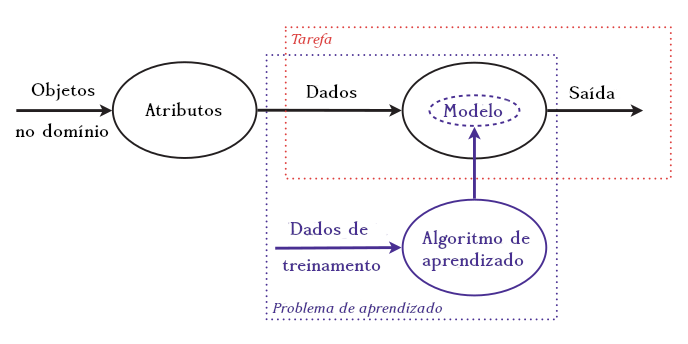
\includegraphics[width=0.8\textwidth]{imgs/tasks}
\end{figure}

O AM é comumente dividido em três paradigmas principais de aprendizado, chamados de aprendizado supervisionado, não-supervisionado e semi-supervisionado. No caso dos algoritmos de aprendizado supervisionado, o objetivo é aprender um mapeamento de entradas para saídas, dado um conjunto rotulado de pares de entradas e saídas. No aprendizado não supervisionado, o algoritmo é apresentado somente aos dados de entrada e o seu propósito é encontrar padrões significativos nos mesmos. O aprendizado semi-supervisionado, por sua vez, normalmente combina uma pequena quantidade de dados rotulados com uma grande quantidade de dados não rotulados para criar um classificador próprio a ser aplicado aos dados não rotulados. Em alguns casos, a abordagem de aprendizado semi-supervisionado pode ser de grande valor prático \cite{khan}.

No caso do paradigma de aprendizado supervisionado, em particular, destacam-se as tarefas de classificação e de regressão. Em uma tarefa de classificação, um algoritmo é selecionado para especificar quais das $k$ categorias possíveis uma entrada pertence. Para resolver essa tarefa, o algoritmo de aprendizado normalmente produz uma função $f : \mathbbm{R}^n \rightarrow \{1, \ldots, k\}$. Quando $y = f(x)$, isto significa que o modelo mapeia uma entrada descrita pelo vetor $x \in \mathbbm{R}^n$ para uma categoria identificado por um valor numérico $y \in \{1, \ldots, k\} $. Quanto à tarefa de regressão, é solicitado a um algoritmo de AM a predição de um valor numérico a partir de uma entrada. Desta forma, o algoritmo de aprendizado é proposto a inferir uma função $f : \mathbbm{R}^n \rightarrow \mathbbm{R}$ \cite{goodfellow}.

 % [Algumas tarefas de regressão podem ser, por exemplo, a determinação do valor de uma corrida de táxi, a identificação da idade de um indivíduo em uma imagem \todo{Citar trabalho da Nicoli}, prever o preço de uma casa baseado nos dados de casas vendidas anteriormente, etc.] \todo{Citar Marsland?} %[Alguns exemplos de tarefa de classificação são a detecção de faces em imagens, a determinação do gênero do indíviduo nessas imagens, a verificação da espécie de uma planta, entre outros.] \todo{Rever exemplos}

Dentre os diversos modelos de AM existentes, Flach considera a categorização dos mesmos segundo os tipos geométricos, probabilísticos e lógicos \cite{flach}. Um modelo geométrico é construído diretamente em função do espaço da solução, utilizando-se de conceitos como linhas, planos, hiperplanos e distâncias. Nesta categoria encontram-se a regressão linear, as redes neurais artificiais e as máquinas de vetores de suporte, por exemplo. Nos modelos do tipo probabilísticos, tendo como exemplo o classificador Bayesiano, a questão principal é modelar a relação entre os dados de entrada e de saída assumindo que existe algum processo aleatório implícito que produz os valores para essas variáveis, de acordo com uma distribuição de probabilidade bem definida', porém desconhecida. Um modelo lógico, por sua vez, é o mais naturalmente algorítmico, considerando a capacidade de ser facilmente transformado em regras que podem ser entendidas por seres humanos. Dentre os modelos lógicos estão, por exemplo, as árvores de decisão e as florestas aleatórias.


\todo[inline]{Construir transição sutil para próxima seção. Sugestão: citar vários exemplos de problemas resolvidos com AM.}
Na próxima seção serão descritas e apresentadas as redes neurais artificias, um dos modelos de AM para o paradigma supervisionado com papel protagonista nas soluções apresentadas.

%%Dentre os modelos geométricos, as redes neurais artificiais têm demonstrado grande desempenho em diversas áreas. Aplicações de \emph{Deep Learning} para detecção de padrões em imagens e reconhecimento de voz, por exemplo, utilizam-se desses modelos para a obtenção de resultados relevantes. Tomando isto e levando em consideração o contexto deste trabalho, as próximas seções apresentadas abordam significativamente estes conceitos.

%%%%%


\section{Redes Neurais Artificiais}
\label{subsec:rna}

As \emph{Redes Neurais Artificiais} (RNAs) são uma tentativa computacional de modelar a capacidade de processamento de informação do sistema nervoso humano \cite{rojas}. Para alcançarem um bom desempenho, as RNAs empregam uma interligação de estruturas bases chamadas de neurônios artificiais que, por sua vez, possuem pesos com valores numéricos positivos ou negativos associados entre si. Uma vantagem das RNAs é a grande capacidade de generalização, ou seja, a habilidade de produzir saídas adequadas para entradas que não estavam presente anteriormente durante seu aprendizado \cite{haykin}. [As RNAs têm sido frequentemente utilizadas nas áreas de processamento de sinais, reconhecimento de padrões em dados, incluindo imagem e voz, medicina, reconhecimento de voz, negócios, entre outras \cite{fausett}. \todo{Olhar Facelli}]

A idealização dos neurônios artificiais foi inspirada nos neurônios biológicos encontrados no cérebro humano. Como mostrado na Figura \ref{fig:sinapse}, cada neurônio biológico é composto pelo corpo celular, os dendritos e o axônio. Os dendritos têm como papel a recepção das informações, ou impulsos nervosos, de outros neurônios e a submissão destas informações ao corpo celular, onde são processadas e novos impulsos são gerados. Estes impulsos são enviados aos dendritos de outros neurônios através do axônio. O ponto de contato entre os neurônios através do axônio e os dentritos, denominado sinapse, é onde ocorre toda a troca de informação necessária para conceber uma rede neural \cite{braga}.

% Procurar nova imagem
\begin{figure}[h!]
\centering
\caption{Estrutura de um neurônio biológico.}
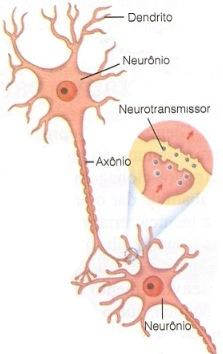
\includegraphics[width=0.25\textwidth]{imgs/sinapse}
\label{fig:sinapse}
\end{figure}
\todo{Refazer imagem livro Teresa}

Considerando uma analogia com os neurônios biológicos, modelou-se então a primeira noção de neurônios artificiais. Nestes neurônios, as entradas são valores $x = x_1, ..., x_n$ aos quais estão sujeitos um conjunto de pesos $w = w_1, ..., w_n$. Este modelo de neurônio utiliza ainda um \emph{bias} externo, denotado por $b$. Este bias é utilizado para o aumentar ou diminuir os valores de entrada da função de ativação, dependendo se o seu valor é positivo ou negativo, respectivamente \cite{haykin}. Um neurônio artificial dispara quando a soma ponderada da entrada e do \emph{bias} sujeita aos pesos ultrapassa um certo limiar de excitação, denominado \emph{threshold}. No modelo de neurônio artificial apresentado, proposto por McCulloch e Pitts (MCP) \cite{mcculloch}, a ativação (disparo) do neurônio é obtida através da aplicação de uma \emph{função de ativação}, como mostrado na Figura \ref{fig:neuronio-artificial} \cite{braga}.

\todo{Ajustar captions}
\begin{figure}[H]
\centering
\caption{Representação de um neurônio artificial. Adaptado de: \cite{haykin}.}
\label{fig:neuronio-artificial}
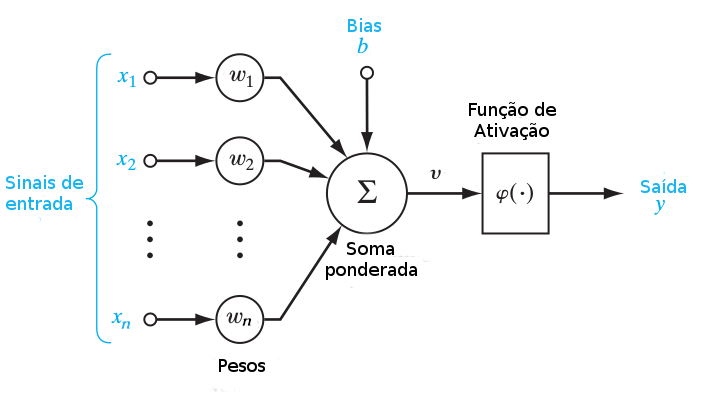
\includegraphics[width=0.8\textwidth]{imgs/neuronio-artificial}
\end{figure}

No caso do neurônio MCP, a função de ativação é do tipo degrau deslocada, conforme Equação \ref{eq:degrau}, e o seu valor de saída é obtido como resultado da comparação entre o \emph{threshold} $\theta$ previamente definido e o valor da soma ponderada da entrada, como mostrado na Equação \ref{eq:soma-ponderada}.

\begin{equation}
\label{eq:degrau}
\varphi(v) = \left\{
\begin{array}{lr}
  1, & \text{se } v > \theta.\\
  0, & \text{caso contrário}.
\end{array}
\right.
\end{equation}

\begin{equation}
  \label{eq:soma-ponderada}
  v = \sum\limits_{i=1}^n x_i w_i + b
\end{equation}


%%Para a correta funcionalidade de determinados algoritmos em RNAs, como o de \emph{backpropagation} em redes \emph{multilayer perceptron}, sabe-se que a escolha da função de ativação deve considerar funções contínuas e diferenciáveis \cite{haykin}.

Embora o modelo MCP tenha considerado apenas funções de ativação do tipo degrau deslocada, outras definições também são possíveis. As funções identidade, sigmóide, tangente hiperbólica e retificada linear (ReLU) são comumente utilizadas, definidas tais como mostrado na Figura \ref{fig:activation}.

\begin{figure}[h!]
  \caption{Exemplos de funções de ativação.}
  \label{fig:activation}
     \subfloat[Identidade ou Linear\label{subfig:identity}]{%
       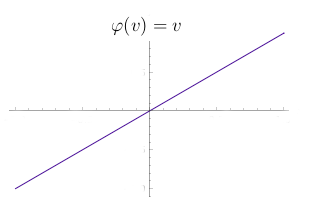
\includegraphics[width=0.4\textwidth]{imgs/identity}
     }
     \hfill
     \subfloat[Tangente Hiperbólica\label{subfig:tanh}]{%
       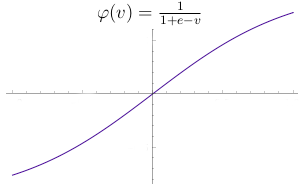
\includegraphics[width=0.4\textwidth]{imgs/tanh}
     }
     \hfill
     \subfloat[Sigmóide ou Logística\label{subfig:sigmoid}]{%
       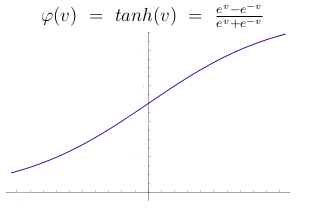
\includegraphics[width=0.4\textwidth]{imgs/sigmoid}
     }
     \hfill
     \subfloat[Unidade Linear Retificada (ReLu)\label{subfig:relu}]{%
       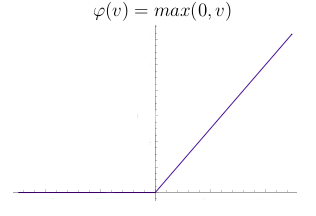
\includegraphics[width=0.4\textwidth]{imgs/relu}
     }
\end{figure}


Em 1958, visando a melhoria do neurônio MCP, Frank Rosenblatt desenvolveu o modelo \emph{Perceptron} \cite{Rosenblatt}. Neste modelo, criou-se o primeiro conceito de aprendizado através de neurônios artificiais, em que foi projetada uma regra de correção de erros para modificar os pesos associados a um neurônio quando suas respostas aos estímulos apresentados ao modelo forem erradas \cite{arbib}. Durante o processo de adaptação à resposta real, deseja-se identificar um valor $\Delta w$ a ser aplicado ao vetor de pesos atual $w(t)$, para que seu valor atualizado $w(t+1)$ esteja mais próximo da solução desejada do que o valor atual $w(t)$. Para isso, definiu-se a Equação \ref{eq:aprendizado1}, denominada Regra Delta, cuja obtenção, descrita na Equação \label{eq:aprendizado2} estabelece o modo detalhado como esse ajuste de pesos é efetuado. Nesta segunda equação, $\eta$ indica uma \emph{taxa de aprendizado}, isto é, a velocidade em que o vetor de pesos será atualizado, e $\hat{y}(t)$ significa o valor previsto pelo modelo naquela iteração para a entrada $x(t)$, enquanto $y(t)$ refere-se à saída real para esta entrada. Desta forma, o neurônio Perceptron adquiriu a capacidade de resolver problemas linearmente separáveis \cite{braga}.

\begin{eqnarray}
  w(t+1) &=& w(t) + \Delta w   \label{eq:aprendizado1}\\
  &=& w(t) + \eta (y - \hat{y}) x(t) \label{eq:aprendizado2}.
\end{eqnarray}

% Arquitetura das redes neurais.
Neurônios artificiais possuem uma capacidade de generalização limitada, independente da função de ativação escolhida, devido a sua habilidade de resolver apenas problemas linearmente separáveis. Entretanto, a combinação desses neurônios para a formação de uma rede é capaz de resolver problemas de elevada complexidade \cite{braga}. Geralmente, identificam-se três classes fundamentais de RNAs, as \emph{feedforward} com uma única camada, as \emph{feedforward} com múltiplas camadas e as recorrentes. Numa rede do tipo \emph{feedforward}, como mostrado nas Figuras \ref{subfig:singlelayer} e \ref{subfig:multilayer}, existe uma camada de entrada que é projetada diretamente para uma camada de saída constituída de neurônios, e nunca ao contrário. Uma rede recorrente, como a na Figura \ref{subfig:recurrent}, por sua vez, possui conexões ponderadas dentro de uma camada e diferencia-se pela presença de pelo menos um loop de retorno a camadas anteriores \cite{haykin}.

% Inserir imagem da topologia das redes com subfig. Haykin ou Faceli.

\begin{figure}[h!]
     \subfloat[\emph{Feedforward} com uma única camada\label{subfig:singlelayer}]{%
       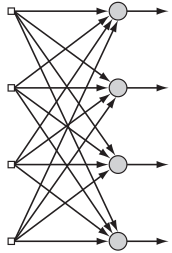
\includegraphics[width=0.25\textwidth]{imgs/feedforward-single}
     }
     \hfill
     \subfloat[\emph{Feedforward} com múltiplas camadas\label{subfig:multilayer}]{%
       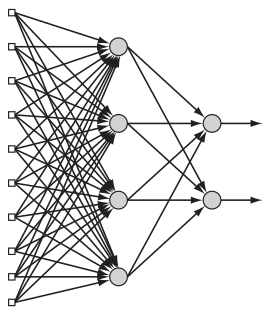
\includegraphics[width=0.35\textwidth]{imgs/feedforward-multi}
     }
     \hfill
     \subfloat[Recorrente\label{subfig:recurrent}]{%
       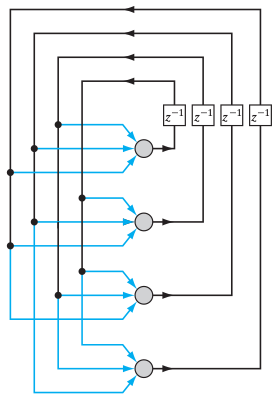
\includegraphics[width=0.3\textwidth]{imgs/recurrent}
     }
     \caption{Arquiteturas populares de RNAs. Fonte: \cite{haykin}}
     \label{fig:architectures}
\end{figure}

Redes com múltiplas camadas, como na Figura \ref{subfig:multilayer}, caracterizam-se pela presença de pelo menos uma camada oculta. Isso acarreta um grande poder às redes deste tipo pois, conforme Cybenko, uma rede com uma camada oculta é capaz de mapear qualquer função contínua, enquanto uma rede com duas camadas ocultas é suficiente para mapear qualquer função \cite{cybenko}.

\subsubsection{\emph{Multilayer Perceptron}}
\label{subsubsec:mlp}

As RNAs do tipo \emph{Multilayer Perceptron} (MLP), são redes constituídas do neurônio Perceptron, \emph{feedforward} e com múltiplas camadas, sendo estas uma camada de entrada, uma ou mais camadas ocultas e uma camada de saída. A arquitetura mais comum para uma rede MLP é a completamente conectada, de forma que os neurônios de uma camada estão conectados a todos os neurônios da próxima camada \cite{faceli}.

Em uma rede MLP, a função implementada por um neurônio de certa camada é uma combinação das funções realizadas pelos neurônios da camada anterior que estão conectados a ele. Na primeira camada, cada neurônio aprende uma função que define um hiperplano. Na camada seguinte, os neurônios combinam um grupo de hiperplanos, formando regiões convexas. Os neurônios da camada seguinte combinam então um subconjunto das regiões convexas em regiões de formato arbitrário \cite{faceli}. Na Figura \ref{fig:aprendizado-mlp}, tem-se uma visualização do processo ocorrido.


\begin{figure}[h!]
\centering
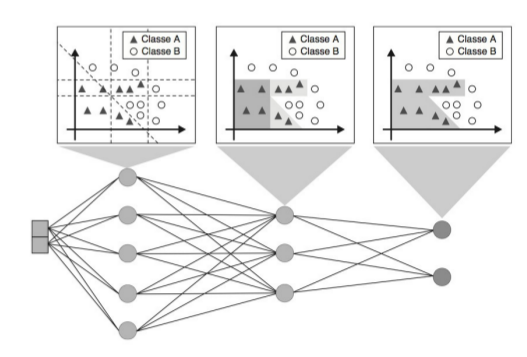
\includegraphics[height=6cm]{imgs/aprendizado-mlp}
\caption{Papel exercido pelos neurônios em cada camada de uma rede MLP. Fonte: \cite{faceli}.}
\label{fig:aprendizado-mlp}
\end{figure}

O algoritmo de aprendizado supervisionado mais conhecido e utilizado para treinamento das MLPs é o \emph{backpropagation}. Neste algoritmo utiliza-se as entradas e as saídas desejadas para o ajuste dos erros da rede. O treinamento ocorre em duas fases, a fase \emph{forward} e a fase \emph{backward}, em que cada fase percorre a rede em um sentido. Na fase \emph{forward}, a saída da rede é definida considerando certo padrão de entrada. A fase \emph{backward} utiliza a saída desejada e a saída fornecida pela rede para atualizar os pesos nas suas conexões \cite{braga}. O \emph{backpropagation} é simplesmente um método que utiliza o gradiente descendente para minimizar o erro quadrático total da saída calculada pela rede, na qual a derivada parcial define o ajuste dos pesos. Essa derivada mede a contribuição de cada peso no erro da rede para a classificação de dado objeto \cite{fausett, faceli}.

% Não tá legal, ajeitar.
No âmbito do cálculo, o gradiente indica o sentido e a direção para os quais devem-se mover os valores dos pesos e do bias nas camadas de forma a garantir o maior incremento possível de perda. Ou seja, nas técnicas de \emph{backpropagation}, queremos mudanças de peso que trarão a inclinação mais íngreme ao longo da função de erro \cite{goodfellow, kubat}.

Um grande crescimento do poder computacional em termos de velocidade e memória tem acontecido nos últimos tempos. Dado isto, houve a viabilidade de treinamento das chamadas \emph{redes neurais profundas}, MLPs que possuem mais camadas escondidas do que o usual. Devido a ampla popularidade dessas redes e a capacidade computacional para a utilização de grande quantidade de dados de treinamento, foram desenvolvidas técnicas de \emph{deep learning} em pleno estado da arte para detecção, segmentação, classificação e reconhecimento de objetos em imagens \cite{khan}. Utilizando-se redes neurais convolucionais, podemos ainda elencar aplicações como o reconhecimento de padrões em imagens para uso na medicina \cite{cha}, a modelagem de frases por computadores \cite{kalchbrenner} e o reconhecimento de caracteres e dígitos \cite{lecun}. Essas e outras técnicas serão apresentadas mais profundamente nas seções a seguir.

%%%%%


\section{\emph{Deep Learning}}
\label{subsec:dl}

\emph{Deep Learning} (DL), também conhecido como Aprendizado Profundo, é uma subárea específica de ML que enfatiza o aprendizado através de sucessivas camadas de representações cada vez mais significativas dos dados submetidos. Estas representações são quase sempre obtidas atráves de redes neurais profundas \cite{chollet}. De acordo com Heaton, qualquer RNA com mais de duas camadas ocultas é, em sua essência, considerada profunda \cite{heaton}. O DL tem obtido um êxito incrível em endereçar problemas de visão computacional e processamento de linguagem natural. Estes algoritmos não só ultrapassaram outras variedades de algoritmos de ML, como também pleiteam a eficácia na classificação alcançada por seres humanos \cite{buduma}.

Os motivos para o corrente sucesso do DL podem ser exemplificados pela grande quantidade de dados disponíveis -- como a base de dados \emph{ImageNet}, organizada conforme a hierarquia \emph{WordNet} e que disponibiliza imagens para pesquisadores ao redor do mundo \cite{imagenet} -- e o custo relativamente baixo de Unidades de Processamento Gráfico (GPUs), que são utilizadas para uma computação numérica muito mais eficiente. Grandes companhias do ramo tecnológico utilizam técnicas de DL diariamente para a análise de enormes quantidades de dados. Entretanto, esta especiliadade não é mais limitada somente ao domínio acadêmico e industrial, ela tornou-se parte integrante da produção de softwares modernos disponibilizados aos consumidores \cite{gulli}.

O DL reúne um conjunto de técnicas e modelos que podem ser aplicados a tarefas de aprendizado supervisionado e não-supervisionado, nas quais as redes neurais convolucionais se destacam expressivamente. A próxima seção descreve os pontos principais relacionados a este tipo de RNA.

\subsubsection{Redes Neurais Convolucionais}
\label{subsubsec:cnns}

As \emph{Redes Neurais Convolucionais} (CNNs, do inglês \emph{Convolutional Neural Networks}) são uma categoria de redes neurais profundas, \emph{feedforward}, que comprovaram ser extremamente bem-sucedidas no ramo de visão computacional \cite{khan}. O termo denominado a estas redes, vem do seu aproveitamento da operação matemática chamada convolução, um tipo especializado de operação linear \cite{goodfellow}. Na Figura \ref{fig:areas-ia} é ilustrada a relação das CNNs com alguns campos de estudos conhecidos.

\begin{figure}[h!]
  \centering
  \caption{A relação entre a visão humana, visão computacional, ML, DL e CNNs. Adaptado de: \cite{khan}.}
  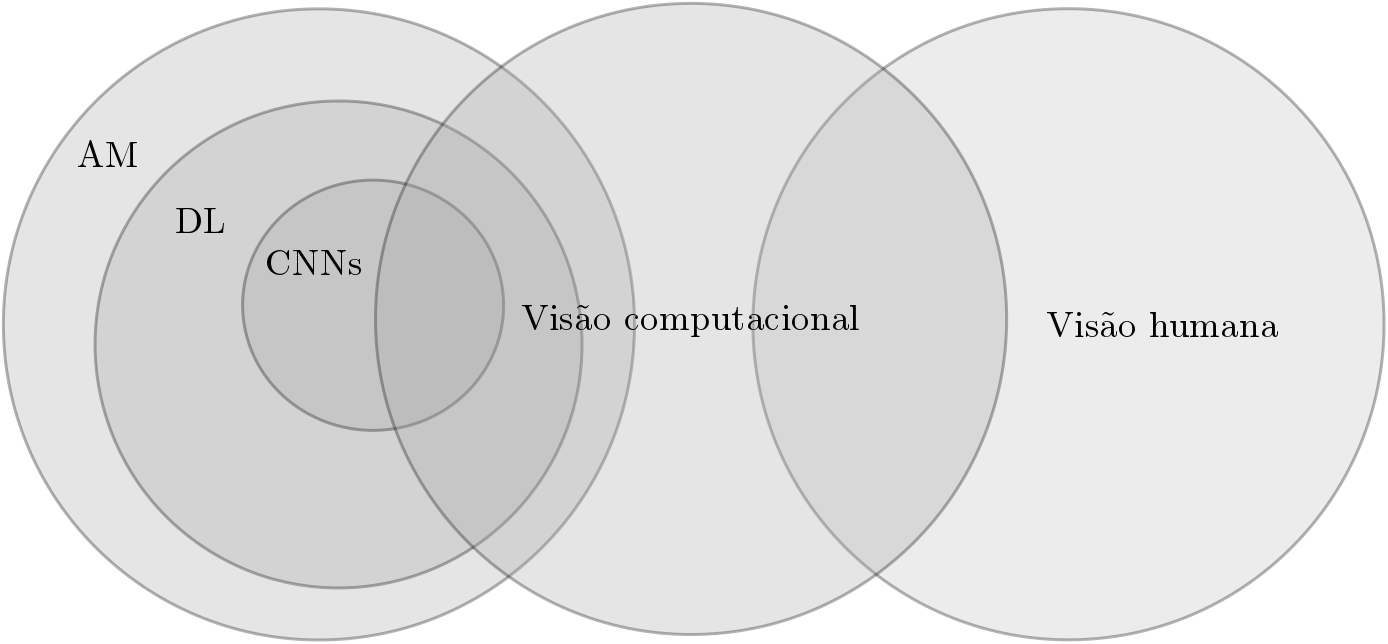
\includegraphics[width=0.7\textwidth]{imgs/areas-ia}
  \label{fig:areas-ia}
\end{figure}

% Convolução
A \emph{convolução} é uma operação que consiste na soma dos produtos de toda a extensão de duas entradas em função de um deslocamento. Sendo assim, a convolução $s(t)$ de duas entradas $x_1(t)$ e $x_2(t)$ é uma função representada simbolicamente por $s(t) = x_1(t) * x_2(t)$ e definidade conforme a Equação \ref{eq:conv} \cite{lathi}.

\begin{equation}
  \label{eq:conv}
  s(t) = x_1(t) * x_2(t) = \int_{-\infty}^{\infty} x_1(\tau)x_2(t - \tau)d\tau
\end{equation}

Nas aplicações de ML, a função $x_1(t)$ é chamada de \emph{input}, a função $x_2(t)$ é o \emph{filtro}, também conhecido como \emph{kernel}, e a saída $s(t)$ consiste no \emph{mapa de características}, gerado pela convolução. O \emph{input} é geralmente uma matriz multidimensional de dados de entrada e o filtro é uma matriz multidimensional de de parâmetros que são ajustados pelo algoritmo de aprendizado. Uma matriz multidimensional no contexto de ML é comumente referenciada como \emph{tensor} \cite{goodfellow}.

As camadas convolucionais são responsáveis por aplicar as operações de convolução. Tomando como exemplo um problema de reconhecimento de padrões em uma imagem, cada camada é responsável por desenvolver os atributos detectados nas camadas anteriores - de linhas, a contornos, a formatos, até construir um objeto por completo. Esse processo pode ser visualizado na Figura \ref{fig:camadas-convolucionais}. Nestas camadas os mapas de características são capturados, e nestes consistem os pesos da rede que são responsáveis por identificar onde são encontrados os atributos na imagem original \cite{buduma}.

\begin{figure}[h!]
\centering
\caption{Processo reproduzido pelas camadas convolucionais de uma CNN, aplicado a um problema de classificação de imagens. Fonte: \cite{khan}.}
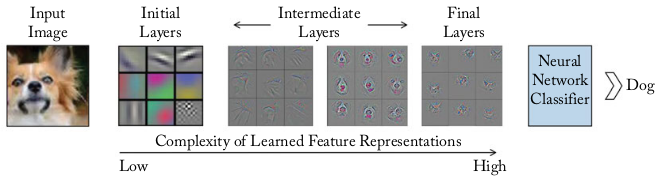
\includegraphics[width=0.9\textwidth]{imgs/camadas-convolucionais}
\label{fig:camadas-convolucionais}
\end{figure}


% Pooling
Uma camada de \emph{pooling} em uma CNN opera em blocos do mapa de características e combina seus atributos através da operação de \emph{max pooling} ou \emph{average pooling}. Esse bloco é deslizado através do mapa de características com um passo definido como \emph{stride}. A operação de \emph{max pooling} retorna o valor máximo dos dados em uma área retangular. Enquanto a operação de \emph{average pooling}, realiza o mesmo processo, porém utiliza a média desses valores. O propósito da camada de \emph{pooling} é, além de diminuir a quantidade de amostras no mapa de características, ajudar a sua representação a se tornar invariante a pequenas mudanças nos dados de entrada \cite{khan, goodfellow}. Uma visualização detalhada dessa operação é demonstrada na Figura \ref{fig:pooling}.

\begin{figure}[h!]
  \centering
  \caption{Visualização da operação de \emph{max pooling} considerando uma região de 2 x 2 com um \emph{stride} igual a 1. Fonte: \cite{khan}.}
  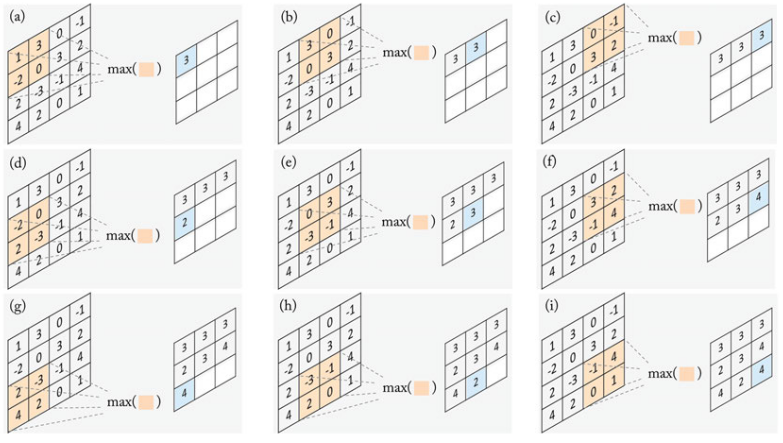
\includegraphics[width=0.8\textwidth]{imgs/pooling}
  \label{fig:pooling}
\end{figure}

% Fully connected layers, camada de saída??

As \emph{Camadas Completamente Conectadas} consideram um conjunto de neurônios completamente conectados aos neurônios da camada anterior, sendo usualmente encontradas no final de uma CNN. Possui a capacidade de separar as variações de classificação que serão retornadas na saída, resumindo os resultados dos vários mapas de características produzidos pela rede \cite{khan}. Na última camada de uma CNN, adota-se geralmente a função de ativação \emph{softmax}, a qual atua escalando as saídas da rede em um vetor de probabilidades, esse processo pode ser muito útil para problemas de classificação \cite{gulli}.

Para prevenir o aprendizado de padrões irrelevantes por um modelo de ML, pode-se articular a quantidade de informações que esse modelo pode armazenar ou adicionar restrições sobre as informações que podem ser armazenadas. Se uma CNN tende a memorizar um pequeno número de padrões, o processo de otimização forçará o foco nos padrões mais proeminentes, que possuem uma chance melhor de gerar uma boa generalização. O processo de evitar o \emph{overfitting} dessa maneira é chamado de \emph{regularização} \cite{chollet}.

O \emph{dropout} é um tipo de regularização muito efetivo e que é usualmente utilizado em CNNs. Consiste na desativação temporária de alguns neurônios durante a fase de treinamento de uma rede. Nesse processo, os neurônios são desativados mediante uma probabilidade $p$, conhecida como \emph{dropout rate}, retornando um valor de saída igual a $0$. Na fase de teste da rede, nenhum neurônio é desativado, ao passo que, como forma de balanceamento devido a quantidade maior de neurônios presentes em comparação à fase de treinamento, os valores de saída das camadas são reduzidos por um fator igual ao \emph{dropout rate} \cite{chollet}. Dessa maneira, pode-se afirmar que o \emph{dropout} ajuda a previnir o \emph{overfitting} ao possibilitar uma forma de combinar diferentes arquiteturas de redes neurais \cite{buduma}. Esta operação pode ser visualizada na Figura \ref{fig:dropout}, na qual os neurônios desativados são demonstrados pelas circunferências com a borda pontilhada.

% Dropout (Pegar imagens sobre Dropout na pagina favoritada )
\begin{figure}[h!]
  \centering
\caption{Processo de aplicação da operação de \emph{dropout}. Os neurônios e ligações desativados estão denotados de forma pontilhada. Fonte: \cite{dsacademy}}
  \subfloat[Arquitetura de uma rede antes da aplicação do \emph{dropout}.\label{subfig:dropout-before}]{%
    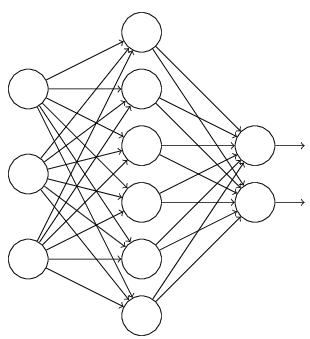
\includegraphics[width=0.4\textwidth]{imgs/dropout-before}
  }
  \hfill
  \subfloat[Arquitetura da rede após a aplicação do \emph{dropout}.\label{subfig:dropout-after}]{%
    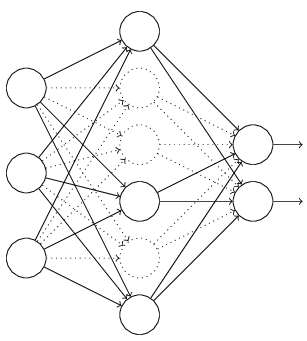
\includegraphics[width=0.4\textwidth]{imgs/dropout-after}
  }
  \label{fig:dropout}
\end{figure}

% Arquiteturas canônicas


\subsubsection{Arquiteturas Canônicas de Redes Neurais Convolucionais}
\label{subsubsec:arq-cnns}

Como mencionado anteriormente, o \emph{ImageNet} é uma base de dados que possui mais de 15 milhões de imagens rotuladas manualmente, de alta resolução, separadas em mais de 22 mil categorias \cite{imagenet}. Visando o uso dessa base, tem sido lançando desde 2010 um desafio anual chamado \emph{ImageNet Large Scale Visual Recognition Challenge} (ILSVRC), no qual possui o intuito de aumentar o desempenho das tecnologias em estado da arte para classificação de imagens e detecção e localização de objetos em imagens \cite{sewak}.

Apesar dos conceitos das camadas que compõem as CNNs serem bastante conhecidos e utilizados, ainda é uma atividade de grande dificuldade e responsabilidade propor arquiteturas de redes neurais que executem determinadas tarefas. Portanto, existem diversas arquiteturas canônicas que apresentam um grande desempenho em treinar e executar tarefas de visão computacional, nas quais a grande maioria foi desenvolvida através do desafio ILSVRC. Devido a grande frequência da utilização dessas arquiteturas, a seguir serão apresentados alguns dos seus aspectos mais relevantes.

A primeira das arquiteturas a ser desenvolvida utilizando camadas convolucionais em vez de camadas completamente conectadas convencionais foi a LeNet, proposta por LeCun em 1998 \cite{lecun}. Uma variante dessa arquitetura é a LeNet-5, composta por sete camadas, nas quais cinco dessas possuem pesos ajustáveis e outras duas são compostas por operações de \emph{max pooling}. Esta arquitetura foi aplicada na identificação de dígitos manuscritos, utilizando o conjunto de dados \emph{Modified National Institute of Standards and Technology} (MNIST) como treinamento. \cite{khan}. Na Figura \ref{fig:lenet} é possível visualizar a composição da LeNet-5.

\begin{figure}[h!]
  \centering
  \caption{A arquitetura LeNet-5. Fonte: \cite{khan}.}
  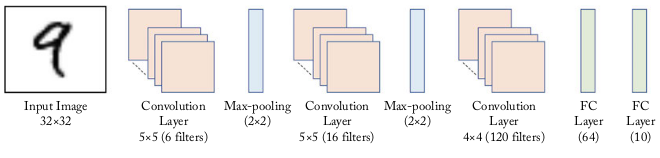
\includegraphics[width=0.8\textwidth]{imgs/lenet5}
  \label{fig:lenet}
\end{figure}

O primeiro modelo em larga escala de CNNs utilizou-se da arquitetura AlexNet, garantindo o primeiro lugar no desafio ILSVRC em 2012 por uma grande margem de diferença dos outros modelos e levando ao ressurgimento da utilização de redes neurais profundas em visão computacional. O uso da função de ativação ReLu após suas oito camadas paramétricas, nas quais as cinco primeiras são convolucionais e as últimas três são completamente conectadas, é um diferencial dessa arquitetura. Operações de \emph{max pooling} são aplicadas após as duas primeiras e a última camada convolucional, ao passo que operações de \emph{dropout} são executadas após as duas primeiras camadas completamente conectadas, acarretando na diminuição do \emph{overfitting} e garantindo uma boa generalização para exemplos não vistos anteriormente \cite{khan}. Apesar de já existirem arquiteturas de CNNs mais eficientes disponíveis, a AlexNet ainda é muito utilizada atualmente, devido a sua estrutura simples e profundidade relativamente menor \cite{sewak}.

\begin{itemize}
  \item LeNet Ok;
  \item AlexNet;
  \item VGGNet
  \item GoogLeNet;
  \item ResNet;
  \item DenseNet.
\end{itemize}


\section{Tecnologias Utilizadas}
\label{subsec:tecnologias}
%!TEX root = ../../main.tex

As tecnologias utilizadas para a realização desse trabalho são, em sua maior parte, relacionadas à linguagem de programação \emph{Python}. A escolha dessa linguagem se dá pela sua popularidade para fins de criação de modelos de ML, assim como a grande quantidade de bibliotecas que facilitam o desenvolvimento desses modelos.

Para o pré-processamento das imagens em termos de redimensionamento e criação dos exemplos dispostos aos modelos, utilizou-se a biblioteca \texttt{PIL} (Pillow) \cite{pillow}. Quanto à manipulação e organização dos arquivos, foram utilizadas as bibliotecas \texttt{os} e \texttt{glob} \cite{os,glob}. A aplicação do treinamento e teste dos modelos propostos ficou por conta das bibliotecas \texttt{keras} e \texttt{tensorflow}\cite{keras, tensorflow}. No que diz respeito ao cálculo de métricas de desempenho, as bibliotecas que tiveram um papel protagonista foram a \texttt{scikit-learn} e a \texttt{numpy}, na qual a última também teve a responsabilidade de manipular o conjunto de imagens e as suas representações matriciais \cite{sklearn,numpy}. Por fim, a visualização dos dados de treinamento e de alguns resultados ficou por conta de biblioteca \texttt{matplotlib} \cite{matplotlib}.

Sabe-se que o treinamento de uma CNN requer um custo computacional muitas vezes não alcançado por unidades de processamento comuns. Portanto, com a finalidade de treinar os modelos propostos, foram utilizadas as GPUs disponíveis no Laboratório de Sistemas Inteligentes da UEA. Porém, durante algumas fases do treinamento das redes, a utilização dos \emph{Kernels} da plataforma \emph{Kaggle} também foram de grande ajuda. Esse recurso permite a utilização de ambientes que facilitam a reprodução de trabalhos relacionados a ciência de dados, possuindo uma grande quantidade de pacotes pré-instalados e a customização de recursos computacionais com GPUs \cite{kaggle}.

